\documentclass[a5paper, 10pt]{article}

% Текст
\usepackage[utf8]{inputenc} % UTF-8 кодировка
\usepackage[russian]{babel} % Русский язык
\usepackage{indentfirst} % красная строка в первом параграфе в главе
% Отображение страниц
\usepackage{geometry} % размеры листа и отступов
\usepackage{listings}
\usepackage{color}

\geometry{
	left=12mm,
	top=25mm,
	right=15mm,
	bottom=17mm,
	marginparsep=0mm,
	marginparwidth=0mm,
	headheight=10mm,
	headsep=7mm,
	nofoot}
\usepackage{afterpage,fancyhdr} % настройка колонтитулов
\pagestyle{fancy}
\fancypagestyle{style}{ % создание нового стиля style
	\fancyhf{} % очистка колонтитулов
	\fancyhead[LO, RE]{Лабораторная работа № 3 } % название документа наверху
	\fancyhead[RO, LE]{ Матрицы в 3D-графике} % название section наверху
	\fancyfoot[RO, LE]{\thepage} % номер страницы справа внизу на нечетных и слева внизу на четных
	\renewcommand{\headrulewidth}{0.25pt} % толщина линии сверху
	\renewcommand{\footrulewidth}{0pt} % толцина линии снизу
}
\fancypagestyle{plain}{ % создание нового стиля plain -- полностью пустого
	\fancyhf{}
	\renewcommand{\headrulewidth}{0pt}
}
\fancypagestyle{title}{ % создание нового стиля title -- для титульной страницы
	\fancyhf{}
	\fancyhead[C]{{\footnotesize
			Министерство образования и науки Российской Федерации\\
			Федеральное государственное автономное образовательное учреждение высшего образования
	}}
	\fancyfoot[C]{{\large 
			Санкт-Петербург, 2023-2024
	}}
	\renewcommand{\headrulewidth}{0pt}
}

% Математика
\usepackage{amsmath, amsfonts, amssymb, amsthm} % Набор пакетов для математических текстов
%\usepackage{dmvnbase} % мехматовский пакет latex-сокращений
\usepackage{cancel} % зачеркивание для сокращений
% Рисунки и фигуры
\usepackage[pdftex]{graphicx} % вставка рисунков
\usepackage{wrapfig, subcaption} % вставка фигур, обтекая текст
\usepackage{caption} % для настройки подписей
\captionsetup{figurewithin=none,labelsep=period, font={small,it}} % настройка подписей к рисункам
% Рисование
\usepackage{tikz} % рисование
\usepackage{circuitikz}
\usepackage{pgfplots} % графики
% Таблицы
\usepackage{multirow} % объединение строк
\usepackage{multicol} % объединение столбцов
% Остальное
\usepackage[unicode, pdftex]{hyperref} % гиперссылки
\usepackage{enumitem} % нормальное оформление списков
\setlist{itemsep=0.15cm,topsep=0.15cm,parsep=1pt} % настройки списков
% Теоремы, леммы, определения...
\theoremstyle{definition}
\newtheorem{Def}{Определение}
\newtheorem*{Axiom}{Аксиома}
\theoremstyle{plain}
\newtheorem{Th}{Теорема}
\newtheorem{Lem}{Лемма}
\newtheorem{Cor}{Следствие}
\newtheorem{Ex}{Пример}
\theoremstyle{remark}
\newtheorem*{Note}{Замечание}
\newtheorem*{Solution}{Решение}
\newtheorem*{Proof}{Доказательство}
% Свои команды
\newcommand{\comb}[1]{\left[\hspace{-4pt}\begin{array}{l}#1\end{array}\right.\hspace{-5pt} } % совокупность уравнений
% Титульный лист
\usepackage{csvsimple-l3}
\newcommand*{\titlePage}{
	\thispagestyle{title}
	\begingroup
	\begin{center}
		%		{\footnotesize
			%			Министерство образования и науки Российской Федерации\\
			%			Федеральное государственное автономное образовательное учреждение высшего образования
			%		}
		%		
		\vspace*{6ex}
		
		{\small
			САНКТ-ПЕТЕРБУРГСКИЙ НАЦИОНАЛЬНЫЙ ИССЛЕДОВАТЕЛЬСКИЙ УНИВЕРСИТЕТ ИТМО	
		}
		
		\vspace*{2ex}
		
		{\normalsize
			Факультет систем управления и робототехники
		}
		
		\vspace*{15ex}
		
		{\Large \bfseries 
			Лабораторная работа № 3
		}
\vspace*{2ex}
	{\Large \bfseries 
			
"Матрицы в 3D-графике "
		}
\vspace*{2ex}
		
		{\normalsize
			по дисциплине Практическая линейная алгебра
		}

	\end{center}
	\vspace*{20ex}
	\begin{flushright}
		{\large 
			\underline{Выполнила}: студентка гр. \textbf{R3238}\\
			\begin{flushright}
				\textbf{Нечаева А. А.}\\
			\end{flushright}
		}
		
		\vspace*{5ex}
		
		{\large 
			\underline{Преподаватель}: \textit{Перегудин Алексей Алексеевич}
		}
	\end{flushright}	
	\newpage
	\setcounter{page}{1}
	\endgroup}

\begin{document}
	\titlePage
	\pagestyle{style}
\newpage




\section{Задание. Создайте кубик.}

\subsection{Как работает код?}
В первой части кода (рисунок 1) задаются координаты вершин куба: каждый столбец -- вершина и сверху вниз в нем заданы координаты $x$, $y$, $z$ в пространстве и $w$ (последняя отвечает за перспективу).
\begin{figure}[h!]
\center{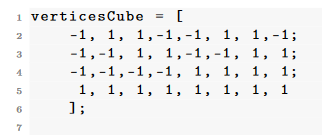
\includegraphics[width=0.5\linewidth]{pic/code1.png}}
\caption{Исходный код кубика, часть 1.}
\end{figure}

Вторая часть (рисунок 2) отвечает за задание плоскостей граней куба, в каждой строчке записаны 4 вершины куба, по которым строится грань.
\begin{figure}[h!]
\center{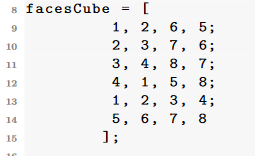
\includegraphics[width=0.5\linewidth]{pic/code2.png}}
\caption{Исходный код кубика, часть 2.}
\end{figure}

Функция $DrawShape$ отвечает за отрисовку кубика, сначала строятся точки вершин по 3 координатам и с учетом перспективы, затем изображаются грани.
\begin{figure}[h!]
\center{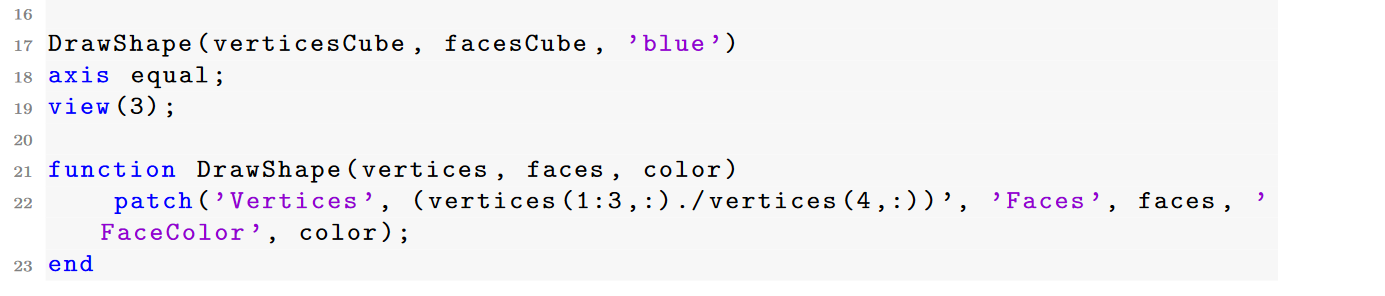
\includegraphics[width=1\linewidth]{pic/code3.png}}
\caption{Исходный код кубика, часть 3.}
\end{figure}

\newpage
\subsection{Почему используется четырехкомпонентный вектор, а не трех?}
Четвертый компонент в векторе позволяет реализовывать перспективную проекцию, а не только отображать ортогональную проекцию. Кроме того, с помощью матрицы $4 \times 4$ реализуются такие преобразования как сдвиги, повороты и т.д. в трехмерном пространстве.

\subsection{Как задать другие фигуры?}






\newpage
\section{Задание. Изменить масштаб кубика.}
Для изменения масштаба кубика использовалась матрица вида:
\begin{equation}
\begin{bmatrix}
a_1 & 0 & 0 & 0\\
0 & a_2 & 0 & 0 \\
0 & 0 & a_3 & 0\\
0 & 0 & 0 & 1
\end{bmatrix}
\end{equation}

Где, $a_1$, $a_2$, $a_3$ отвечают за изменение масштаба по $x$, $y$ и $z$ соответственно.
\begin{figure}[h!]
\center{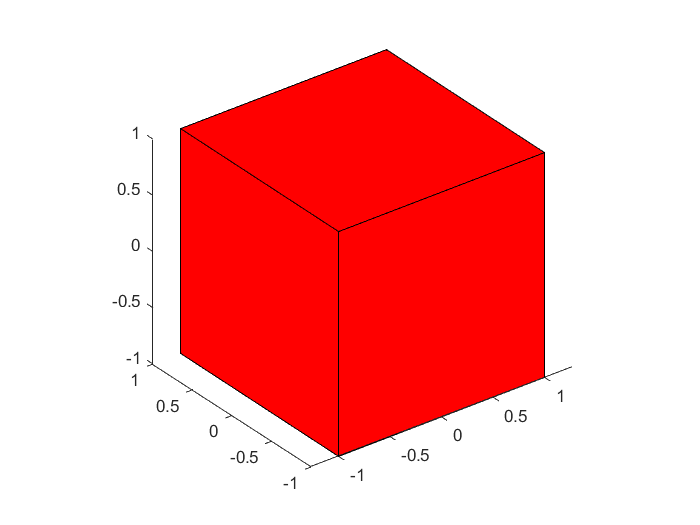
\includegraphics[width=1\linewidth]{pic/task_2_1.png}}
\caption{Оригинальный масштаб,при $a_i = 1$ .}
\end{figure}

\begin{figure}[h!]
\center{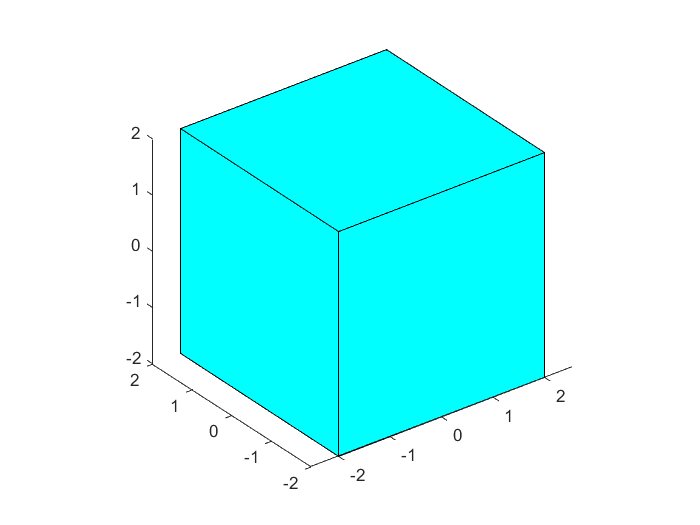
\includegraphics[width=0.75\linewidth]{pic/task_2_2.png}}
\caption{Результат при $a_i = 2$ .}
\end{figure}

\newpage
\begin{figure}[h!]
\center{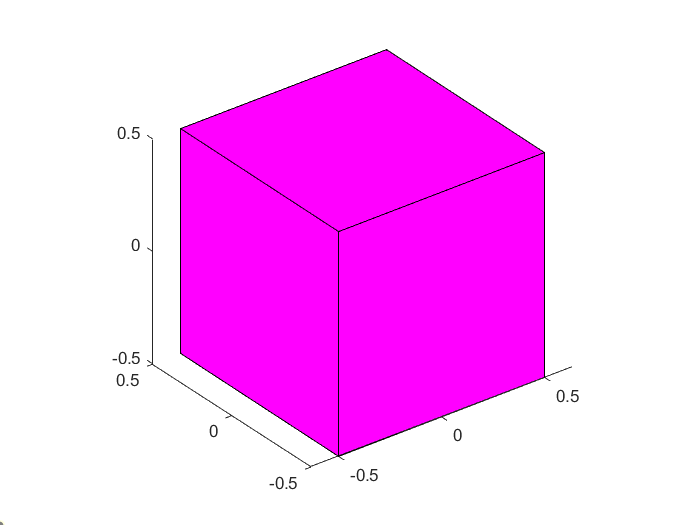
\includegraphics[width=0.75\linewidth]{pic/task_2_3.png}}
\caption{Результат при $a_i = 0.5$ .}
\end{figure}

\newpage
\begin{figure}[h!]
\center{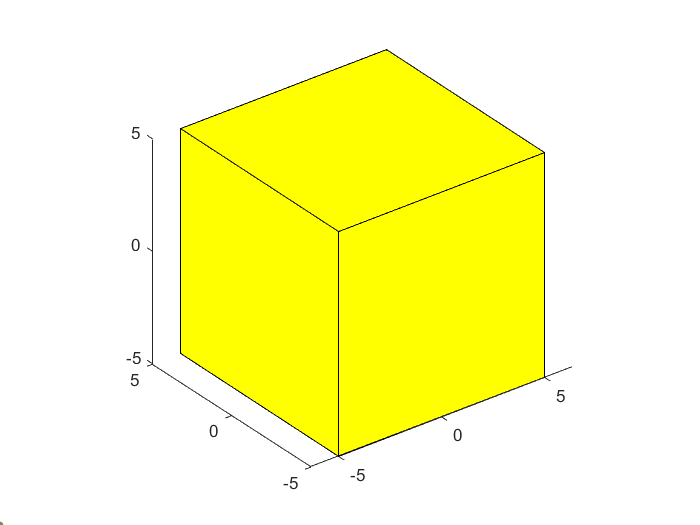
\includegraphics[width=0.75\linewidth]{pic/task_2_4.png}}
\caption{Результат при $a_1 = 15, \, a_2 = 10, \, a_3 = 5$ .}
\end{figure}

\begin{center}
\begin{lstlisting}
sizeMatrix = [
    15, 0, 0, 0;
    0, 10, 0, 0;
    0, 0, 5, 0;
    0, 0, 0, 1
    ];

newVertices = sizeMatrix * verticesCube;

DrawShape (newVertices, facesCube, 'y')
\end{lstlisting}
\textit{Листинг 1. Часть кода, отвечающая за масшабирование кубика.}
\end{center}



\newpage
\section{Задание. Переместить кубик.}
Для перемещения кубика используется матрица вида:
\begin{equation}
\begin{bmatrix}
1 & 0 & 0 & b_1\\
0 & 1 & 0 & b_2 \\
0 & 0 & 1 & b_3\\
0 & 0 & 0 & 1
\end{bmatrix}
\end{equation}
Сдвиг осуществляется на вектор $(b_1, \, b_2, \, b_3)$, подобная операция возможна из-за наличия четвертой координаты точки, так как она умножается на $b_i$ и складывается с $x$, $y$, или $z$:

\begin{equation}
\begin{bmatrix}
1 & 0 & 0 & b_1\\
0 & 1 & 0 & b_2 \\
0 & 0 & 1 & b_3\\
0 & 0 & 0 & 1
\end{bmatrix}
\begin{bmatrix}
x\\
y\\
z\\
1
\end{bmatrix}
=
\begin{bmatrix}
x + b_1\\
y + b_2\\
z + b_3\\
1
\end{bmatrix}
\end{equation}


\begin{figure}[h!]
\center{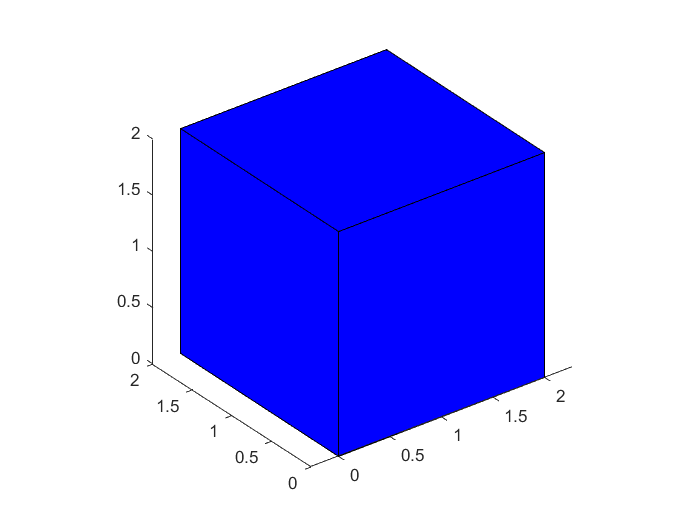
\includegraphics[width=0.75\linewidth]{pic/task_3_1.png}}
\caption{Сдвиг графика на вектор $(1, 1, 1)$.}
\end{figure}

\newpage
\begin{center}
\begin{lstlisting}
moveMatrix = [
    1, 0, 0, 2;
    0, 1, 0, 3;
    0, 0, 1, 4;
    0, 0, 0, 1
    ];

newVertices = moveMatrix * verticesCube;

DrawShape (newVertices, facesCube, 'y')
\end{lstlisting}
\textit{Листинг 2. Часть кода, отвечающая за перемещение кубика.}
\end{center}

Применим последовательно операции масштабирования и перемещения кубика:

\begin{figure}[h!]
\center{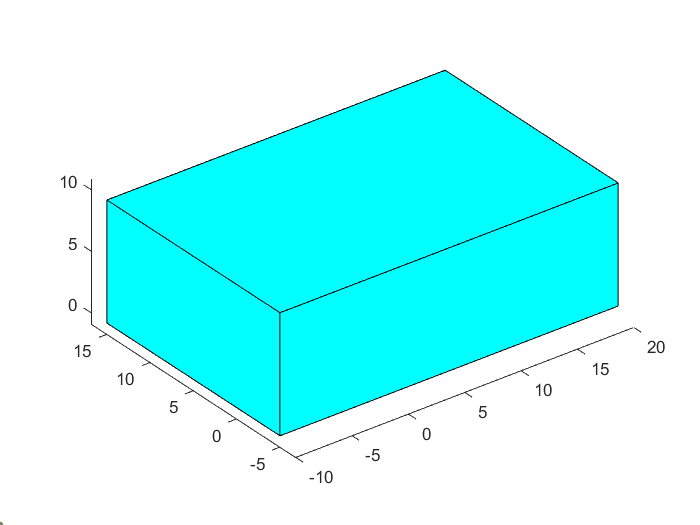
\includegraphics[width=0.75\linewidth]{pic/task_3_2.png}}
\caption{Масштабирование при $a_1 = 15, \, a_2 = 10, \, a_3 = 5$ и сдвиг графика на вектор $(5, 5, 5)$.}
\end{figure}
\newpage
\begin{center}
\begin{lstlisting}
moveMatrix = [
    1, 0, 0, 5;
    0, 1, 0, 5;
    0, 0, 1, 5;
    0, 0, 0, 1
    ];

sizeMatrix = [
    15, 0, 0, 0;
    0, 10, 0, 0;
    0, 0, 5, 0;
    0, 0, 0, 1
    ];

newVertices = moveMatrix * sizeMatrix * verticesCube;

DrawShape (newVertices, facesCube, 'c')
\end{lstlisting}
\textit{Листинг 3. Часть кода, отвечающая за масштабирование и перемещение кубика.}
\end{center}
Заметим, что для получения корректного результата важен порядок умножения матриц: сначала кубик масшабируется, а затем сдвигается, то есть $newVertices = moveMatrix * (sizeMatrix * verticesCube) = moveMatrix *sizeMatrix * verticesCube$.\\
Если сначала выполнить сдвиг, а после -- масшабирование, то матрица сдвига тоже будет влиять на масштаб результата.

\newpage
\section{Задание. Выполнить вращение кубика.}
Матрица вращения определена для каждой оси в $3D$ пространстве. Пусть угол поворота $\phi$.\\
Матрица вращения вокруг оси $X$:

\begin{equation}
\begin{bmatrix}
1 & 0 & 0 & 0\\
0 & \cos \phi & - \sin \phi & 0 \\
0 & \sin \phi & \cos \phi & 0\\
0 & 0 & 0 & 1
\end{bmatrix}
\begin{bmatrix}
x\\
y\\
z\\
1
\end{bmatrix}
=
\begin{bmatrix}
x \\
y \cos \phi - z \sin \phi \\
y \sin \phi + z \cos \phi\\
1
\end{bmatrix}
\end{equation}

Матрица вращения вокруг оси $Y$:

\begin{equation}
\begin{bmatrix}
 \cos \phi & 0 & \sin \phi & 0\\
0 & 1 & 0 & 0 \\
- \sin \phi & 0 & \cos \phi & 0\\
0 & 0 & 0 & 1
\end{bmatrix}
\begin{bmatrix}
x\\
y\\
z\\
1
\end{bmatrix}
=
\begin{bmatrix}
x \cos \phi + z \sin \phi \\
y \\
-x \sin \phi + z \cos \phi\\
1
\end{bmatrix}
\end{equation}

Матрица вращения вокруг оси $Z$:

\begin{equation}
\begin{bmatrix}
 \cos \phi & - \sin \phi & 0 & 0\\
\sin \phi & \cos \phi & 0 & 0 \\
0 & 0 & 1 & 0\\
0 & 0 & 0 & 1
\end{bmatrix}
\begin{bmatrix}
x\\
y\\
z\\
1
\end{bmatrix}
=
\begin{bmatrix}
x \cos \phi - y \sin \phi \\
x \sin \phi + y \cos \phi \\
 z \\
1
\end{bmatrix}
\end{equation}

Вращение по нескольким осям может привести к \textit{проблеме шарнирного замка}, поэтому обычно используется вращение вокруг конкретной оси, например заданную вектором $ \left( \frac{1}{\sqrt{3}}, \frac{1}{\sqrt{3}}, \frac{1}{\sqrt{3}} \right) $, ось должна быть задана единичным вектором.\\
В данной работе будем проводить вращение относительно осей  $X$,  $Y$,  $Z$:

\begin{center}
\begin{lstlisting}
phi = pi/3;

rotateXMatrix = [
    1, 0, 0, 0;
    0, cos(phi), -sin(phi), 0;
    0, sin(phi), cos(phi), 0;
    0, 0, 0, 1 ];

newVertices = rotateXMatrix * verticesCube;
DrawShape (newVertices, facesCube, 'c')
\end{lstlisting}
\textit{Листинг 4. Часть кода, вращение кубика вокруг оси $X$ на 60\textdegree}
\end{center}

\begin{figure}[h!]
\center{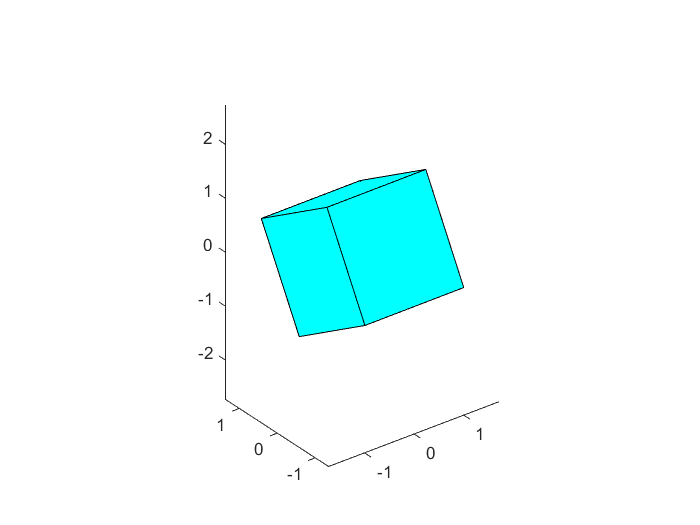
\includegraphics[width=0.75\linewidth]{pic/task_4_1.png}}
\caption{Вращение кубика вокруг оси $X$ на 60\textdegree.}
\end{figure}

\begin{figure}[h!]
\center{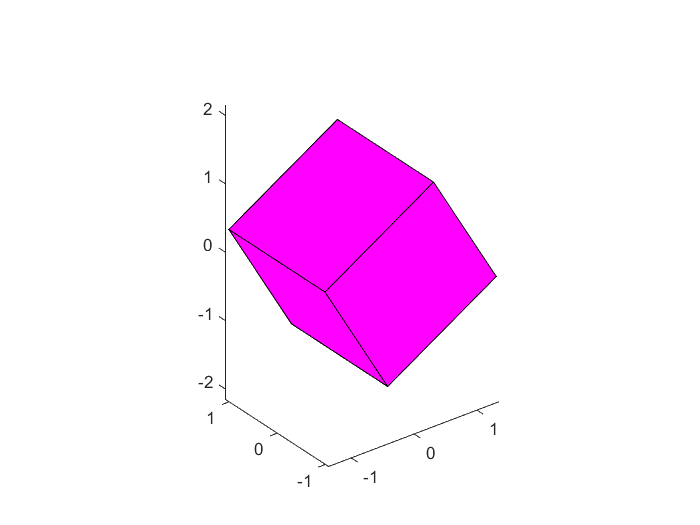
\includegraphics[width=0.75\linewidth]{pic/task_4_2.png}}
\caption{Вращение кубика вокруг оси $Y$ на 60\textdegree.}
\end{figure}

\begin{figure}[h!]
\center{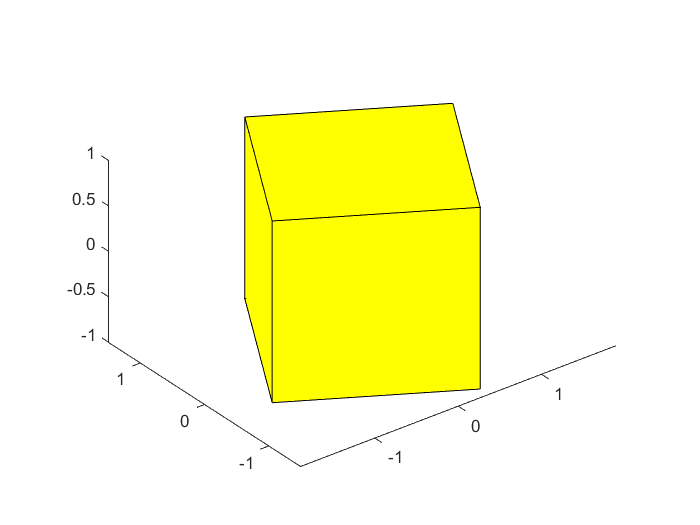
\includegraphics[width=0.5\linewidth]{pic/task_4_3.png}}
\caption{Вращение кубика вокруг оси $Z$ на 60\textdegree.}
\end{figure}

Построить комбинации поворотов. Относительно оси $X$, затем $Y$:
\begin{figure}[h!]
\center{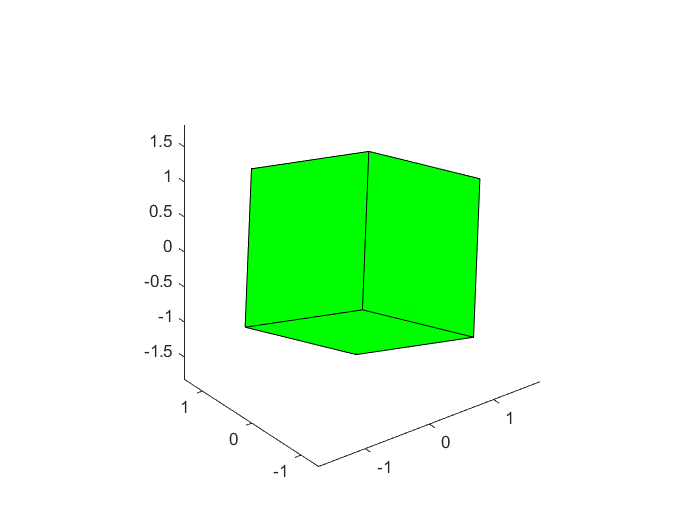
\includegraphics[width=0.75\linewidth]{pic/task_4_4.png}}
\caption{Вращение кубика вокруг оси $X$ на 60\textdegree, затем $Y$ на 30\textdegree .}
\end{figure}

\newpage
Теперь поменяем порядок:
\begin{figure}[h!]
\center{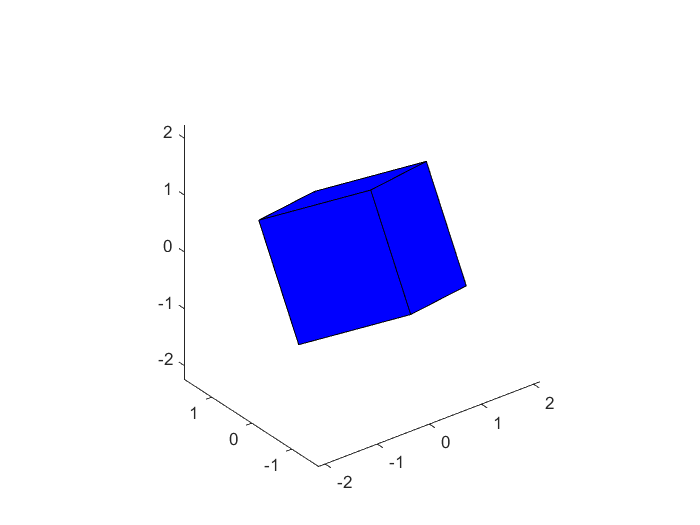
\includegraphics[width=0.75\linewidth]{pic/task_4_5.png}}
\caption{Вращение кубика вокруг оси $Y$ на 30\textdegree, затем $X$ 60\textdegree.}
\end{figure}

\newpage
\section{Задание. Выполнить вращение кубика около одной вершины.}



\newpage
\section{Задание. Реализация камеры.}


\newpage
\section{Задание. Реализация перспективы.}



\newpage
\section{Задание. * Почти Minecraft.}



Для визуализации был написан код на языке \textit{Python} с использованием библиотек \textit{Matplotlib} и \textit{Numpy}. \\
Код расположен на \href{https://github.com/a-nechaeva/practical_Linal/tree/main/lab2/py_code}{\textbf{GitHub}}.
\\
\textit{Отражение (симметрию) плоскости относительно прямой $y=ax$, в нашем случае после подстановки $a=2$, получаем $y=2x$. Задача -- найти матрицу вида}:


\end{document}













